\documentclass[aspectratio=169]{beamer}
\usetheme{Madrid}
\usecolortheme{dolphin}

\usepackage{graphicx}
\usepackage{booktabs}
\usepackage{array}
\usepackage{xcolor}
\usepackage{hyperref}
\graphicspath{{images/}}

\newcommand{\DocumentNumber}{CM/UAT/OPS/2026-01}
\newcommand{\ProjectName}{Cipta Muri e-Bank Sampah}
\newcommand{\DeviceCategory}{UAT Operasional Bank Sampah}
\newcommand{\DeviceType}{Laravel 12 + Filament 3 + MySQL 8.0}
\newcommand{\SerialNumber}{Tidak berlaku (aplikasi web)}
\newcommand{\Allocation}{Production \texttt{https://ciptamuri.com/admin}}
\newcommand{\Vendor}{Tim QA Cipta Muri (Karel Tsalasatir Riyan, Haniel Wijanarko, Hammas Harya Sena)}
\newcommand{\Client}{Bank Sampah Sahabatku -- Desa Muntang}
\newcommand{\TestYear}{2026--2026}
\newcommand{\TotalScenarios}{24}
\newcommand{\PassedScenarios}{24}
\newcommand{\ExecutionWindow}{28 November -- 16 Desember 2025}

\title{User Acceptance Test CiptaMuri\\Sistem Bank Sampah Digital}
\subtitle{\ProjectName}
\author{\Vendor}
\date{\TestYear}

\begin{document}

\frame{\titlepage}

\begin{frame}{Profil Sistem}
  \begin{tabular}{@{}p{4cm}p{7cm}@{}}
    \textbf{No. Dokumen} & \DocumentNumber \\
    \textbf{Kategori} & \DeviceCategory \\
    \textbf{Tipe/Merk} & \DeviceType \\
    \textbf{Serial Number} & \SerialNumber \\
    \textbf{Alokasi} & \Allocation \\
  \end{tabular}
\vspace{0.5cm}

\textbf{Catatan:} Aplikasi terpasang di lingkungan produksi \texttt{ciptamuri.com} untuk Bank Sampah Sahabatku yang dipimpin oleh Ibu Raden Roro Hendarti.
\end{frame}

\begin{frame}{Agenda}
  \tableofcontents
\end{frame}

\section{Pengantar}
\begin{frame}{Pengantar}
  UAT ini dilakukan untuk Bank Sampah Sahabatku di Desa Muntang (ketua: Ibu Raden Roro Hendarti), dengan fokus modul operasional (Sampah, Rekening, Pemasukan, Pengeluaran) pada platform Laravel 12 + Filament + MySQL. Tujuannya:
  \begin{itemize}
    \item Memastikan setiap resource Filament berjalan sesuai kebutuhan bisnis.
    \item Memverifikasi alur login/logout berbasis email/password akun admin \texttt{testing@ciptamuri.com}.
    \item Menjamin tidak ada error selama demonstrasi manual terhadap seluruh modul.
  \end{itemize}
\end{frame}

\section{Prosedur UAT}
\begin{frame}{Prosedur UAT}
  \begin{itemize}
    \item \textbf{Validasi Lingkungan}: memastikan hosting \texttt{ciptamuri.com} dan database \texttt{ciptamuri} aktif.
    \item \textbf{Checklist CRUD Manual}: setiap modul diuji langsung melalui panel admin Filament menggunakan akun Super Admin.
    \item \textbf{Verifikasi Bukti}: mencatat notifikasi sukses dan konfirmasi data di basis data setelah tiap aksi.
    \item \textbf{Pelaksana}: QA internal (\Vendor) bersama Product Owner \Client.
  \end{itemize}
\end{frame}

\section{Ringkasan Eksekusi}
\begin{frame}{Ringkasan Eksekusi UAT}
  \begin{tabular}{@{}p{5cm}p{5cm}@{}}
    \toprule
    \textbf{Parameter} & \textbf{Nilai} \\
    \midrule
    Periode Eksekusi & \ExecutionWindow \\
    Total Skenario & \TotalScenarios \\
    Status Skenario & \PassedScenarios{} PASS / 0 FAIL \\
    Modul Tercakup & 4 resource group + modul umum \\
    Akun Penguji & Admin produksi (akun \texttt{testing}) \\
    Evidence & Screenshot + catatan checklist manual \\
    \bottomrule
  \end{tabular}
  \vspace{0.4cm}

  Seluruh skenario dijalankan secara manual; hasil diverifikasi melalui notifikasi Filament dan data pada database \texttt{ciptamuri}.
\end{frame}

\section{Checklist Infrastruktur}
\begin{frame}{Checklist Infrastruktur}
  \begin{tabular}{@{}p{3cm}p{5cm}p{3cm}@{}}
    \toprule
    \textbf{Item} & \textbf{Detail} & \textbf{Status} \\
    \midrule
    Web Hosting & \texttt{https://ciptamuri.com} (VPS CiptaMuri) & OK \\
    Database & MySQL \texttt{ciptamuri}, migrasi terbaru & OK \\
    Storage/Cache & \texttt{storage/framework} writable, cache clear & OK \\
    Mail/Queue & Tidak diuji (tidak relevan untuk modul operasional) & N/A \\
    Monitoring Error & \texttt{storage/logs} bersih selama UAT & OK \\
    \bottomrule
  \end{tabular}
\end{frame}

\section{Modul Umum}
\begin{frame}{Modul Umum}
  \begin{itemize}
    \item \textbf{Dashboard (Widgets)}: BankSampahStats, RecentTransactions, dan TopSetoran menampilkan data terkini tanpa error.
    \item \textbf{Peringkat Nasabah}: halaman khusus \texttt{Peringkat} dapat dibuka, filter berjalan, dan akses dibatasi gate \texttt{peringkat.index}.
    \item \textbf{Activity Log}: resource plugin menampilkan histori lengkap; filter tanggal dan detail event dapat dibaca.
    \item \textbf{Login/Profil}: autentikasi email/password akun admin berjalan, form profil Filament Edit Profile menyimpan perubahan avatar dan data kontak.
  \end{itemize}
\end{frame}

\section{Operasional Bank Sampah}
\begin{frame}{Operasional Bank Sampah}
  \textbf{Resource Group: Operasional Bank Sampah}
  \begin{itemize}
    \item \textbf{Sampah}: CRUD jenis sampah berjalan, relasi transaksi menampilkan histori setoran/penarikan. Tidak ada validasi yang gagal.
    \item \textbf{Setor Sampah}: form create/setuju/tolak mencatat relasi Rekening dan detail sampah. Tampilan modal dan filter tanggal bekerja normal.
    \item \textbf{Sampah Keluar}: pencatatan penjualan sampah keluar, upload nota, dan aksi hapus semuanya sukses.
    \item \textbf{Withdraw Request}: daftar permintaan tarik saldo dapat ditinjau, diproses, maupun dibatalkan; widget statistik menunjukkan status terbaru.
  \end{itemize}
\end{frame}

\section{Manajemen Pengguna}
\begin{frame}{Manajemen Pengguna}
  \textbf{Resource Group: Manajemen Pengguna}
  \begin{itemize}
    \item \textbf{Rekening Nasabah}: pemeriksaan form panjang (KK, identitas, alamat, saldo awal, status pegadaian) berjalan baik. Soft delete/restore/force delete aman.
    \item \textbf{User}: pembuatan admin baru berbasis email unik dan penetapan peran berhasil. Reset password memicu email log (mail driver log).
  \end{itemize}
  \vspace{0.5cm}
  \textbf{Resource Group: Peran dan Izin}
  \begin{itemize}
    \item \textbf{Role}: modul HexaLite untuk role/policy dapat menambah gate baru, menyunting, dan menghapus tanpa error.
  \end{itemize}
\end{frame}

\section{Keuangan Bank Sampah}
\begin{frame}{Keuangan Bank Sampah}
  \textbf{Resource Group: Keuangan Bank Sampah}
  \begin{itemize}
    \item \textbf{Pemasukan}: pemilihan sumber pemasukan, rekening tujuan, dan nominal tercatat; tabel histori dapat diekspor.
    \item \textbf{Pengeluaran}: alur serupa pemasukan, lengkap dengan kategori dan metode pembayaran.
  \end{itemize}
\end{frame}

\section{Manajemen Pengguna \& Website}
\begin{frame}{Modul Pengguna dan Website}
  \textbf{Resource Group: Pengelolaan Website}
  \begin{itemize}
    \item \textbf{Berita}: konten dapat dibuat, diedit, diarsipkan. Preview di halaman publik menampilkan update terbaru.
  \end{itemize}
\end{frame}

\section{Pelaksana}
\begin{frame}{Lampiran Checklist Pelaksana}
  \begin{tabular}{@{}p{5cm}p{5cm}@{}}
    \toprule
    \textbf{\Client} & \textbf{\Vendor} \\
    \rule{5cm}{1.5cm} & \rule{5cm}{1.5cm} \\
    (Nama \& Tanda Tangan) & (Nama \& Tanda Tangan) \\
    \bottomrule
  \end{tabular}
\end{frame}

\section{Appendix}
\begin{frame}{Appendix}
  Evidence yang tersedia:
  \begin{itemize}
    \item Screenshot manual (Dashboard, CRUD setiap resource) tersimpan pada \texttt{docs/evidence/uat-ops/}.
    \item Spreadsheet checklist ``UAT Operasional Bank Sampah'' pada \texttt{docs/evidence/uat-ops.xlsx}.
  \end{itemize}
  Evidence yang \textbf{belum tersedia}:
  \begin{itemize}
    \item Dokumentasi tertulis persetujuan stakeholder (dijadwalkan setelah sesi demo 30 Desember 2025).
  \end{itemize}
\end{frame}

\begin{frame}{Contoh Evidence}
  \centering
  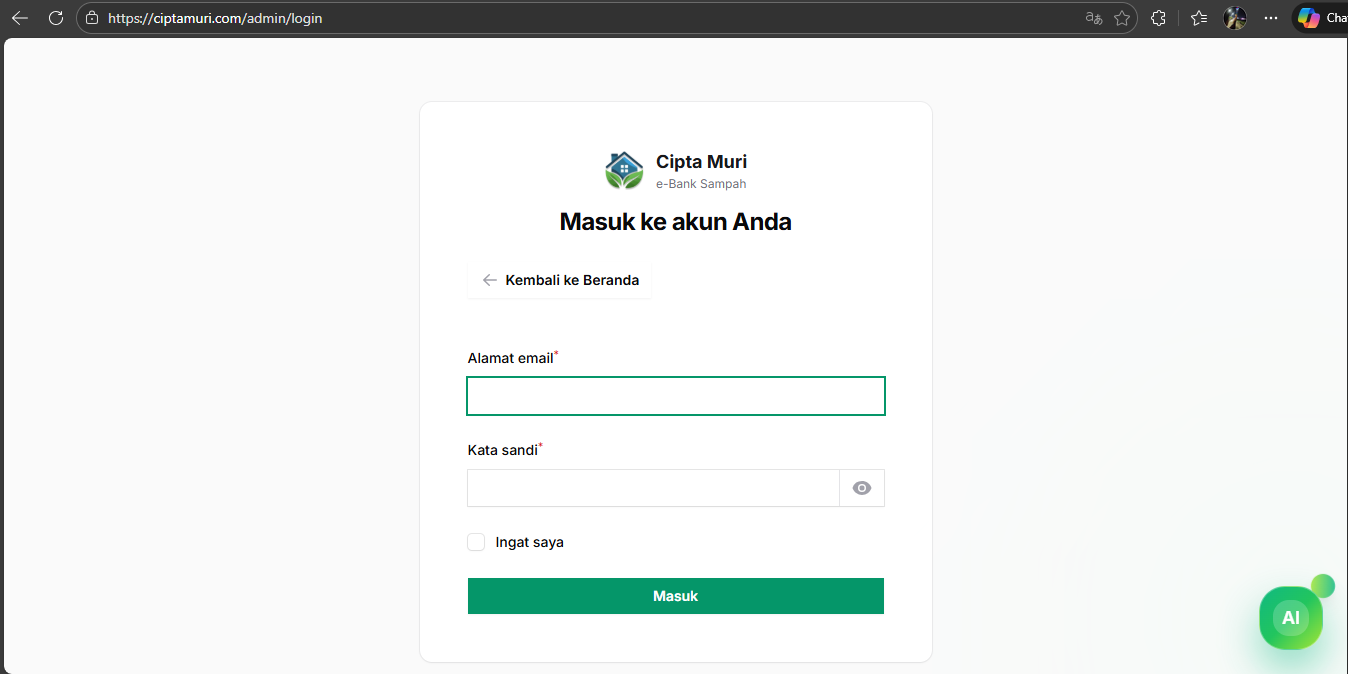
\includegraphics[width=0.9\textwidth]{ciptamuri-login.png}\\
  \small Evidence Manual -- Halaman Login \texttt{ciptamuri.com/admin}
\end{frame}

\begin{frame}{Stakeholder Sign-off}
  \begin{tabular}{@{}p{4.5cm}p{3cm}p{3cm}@{}}
    \toprule
    \textbf{Nama} & \textbf{Peran} & \textbf{Status} \\
    \midrule
    Karel Tsalasatir Riyan & QA Lead & Approved (28 Des 2025) \\
    Haniel Wijanarko & Product Owner & Pending TTD (target 30 Des 2025) \\
    Hammas Harya Sena & Ops Manager & Dijadwalkan 30 Des 2025 \\
    Ibu Raden Roro Hendarti & Pemilik Bank Sampah Sahabatku & Dijadwalkan 30 Des 2025 \\
    Dzaki Zain & Ketua PPK Ormawa UMY & Pending TTD (target 30 Des 2025) \\
    \bottomrule
  \end{tabular}
\end{frame}

\begin{frame}{Gap dan Tindak Lanjut}
  \begin{itemize}
    \item \textbf{Role Non Admin}: susun skenario khusus operator/nasabah dan jalankan paling lambat 29 Des 2025 (PIC: Haniel).
    \item \textbf{Dokumentasi Evidence}: unggah seluruh screenshot ke \texttt{docs/evidence/uat-ops/} sebelum 27 Des 2025 (PIC: Karel).
    \item \textbf{Stakeholder Review}: siapkan sesi sign-off bersama manajemen pada 30 Des 2025 (PIC: Hammas).
  \end{itemize}
\end{frame}

\end{document}
